\section{Infrastructure}
In this chapter we will discuss our infrastructure setup for building and
running ConAir, and the toolchain of using the ConAir tool.

\subsection{Infrastructure Setup}
One of the standards that was mentioned previously to evaluate the tool is
Compatibility, which means the tool should have no OS/hardware modification.
When we try to build and run the ConAir tool, however, we find out that although
it does not require any OS/hardware modification, it has very strong requirement
to the OS and corresponding software installed.

We make many effort in order to make Conair compile and run. For example, We try
four different versions of Linux: Ubuntu 12.04 x64, Ubuntu 12.04 x86, the
Lonestar Cluster of UT, as well as CentOS 5.9. The first two are the OS that we
have as a virtual machine. None of them work perfectly. Then we ask the
author and they provide us the specific OS version that they use. Then we try
Lonestar Cluster which has an OS pretty similar to the one that the author
provides, but we do not have the previlidge to install the required runtime
library. Finally we tried CentOS 5.9 which is exactly the same as the author
suggests, but we still cannot fix the compatibility issue (missing GLIBCXX\_3.4.9
and GLIBC\_2.7).

We also try different versions of LLVM, llvm-gcc and gcc. Specifically, we try
two versions of LLVM, llvm-2.8 and llvm 2.9; we try three versions of llvm-gcc:
the binary of llvm-gcc-4.2-2.8, binary of llvm-gcc-4.2-2.9, and llvm-gcc-4.2-2.8
built from source code; also we try five different versions of gcc: 4.7.3,
4.6.3, 4.4.3, 4.2.1 and 4.3.1 from source. For each try we do our best to remove
any compilation or dependency issue, and we try many combination between
different OS, LLVM, llvm-gcc and gcc. This process is very tedious and it take
more than 50\% of our time for this project. However, although we try very hard
we still cannot find a combination that is perfectly working. The main problem
we face is that the front end of LLVM cannot treat floating point global
variables appropriately. We believe that is because the version of LLVM we use
is too old, but ConAir does not support newer version of LLVM.

Fortunately, although we have the above issue, for normal multithread programs
without floating points we are able to make ConAir compile and run. Therefore we
can still do some experiments to demonstrate the effect of ConAir. We will show
our experiment results in section~\ref{sec:experiment}

\subsection{Toolchain}
There are several steps needed to make ConAir work, and
Figure~\ref{fig:toolchain} shows the structure of the ConAir ToolChain. Here we
want to generate two executables, the original one and the fixed one, so that we
can compare and see if the concurrency bugs have been fixed or not.\\
\begin{figure}[htbp]
\centering
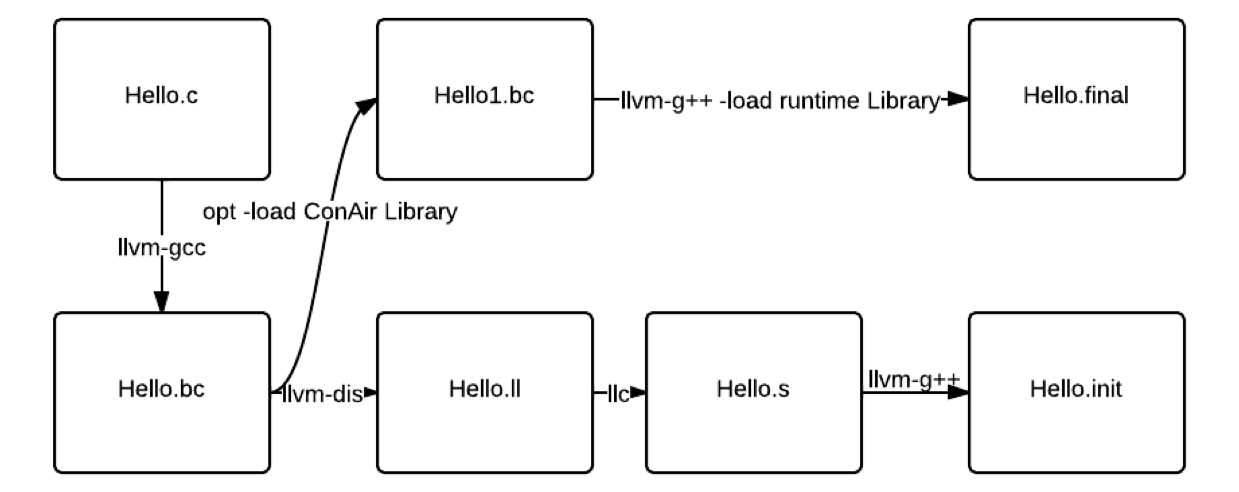
\includegraphics[width=0.5\textwidth]{figs/toolchain.png}
\caption{Toolchain of ConAir}
\label{fig:toolchain}
\end{figure}
\textbf{Generating the original executable}
In order to generate the original executable, we first use \textbf{llvm-gcc}, a
LLVM front end compiler, to compile the C source code \textit{Hello.c}, into
LLVM bitcode \textit{Hello.bc}. LLVM bitcode is a high level intermediate
representaton (IR) of LLVM. It will unify source code in different languages
into a common source code, with no optimization applied.

After the LLVM bitcode is generated, we then use \textbf{llvm-dis}, a LLVM
diassembler, to diassemble the above bitcode into LLVM assembly code
\textit{Hello.ll}. After that, we will use \textbf{llc}, a static compiler of
llvm, to generate the above assembly code into another assembly code for a
specified architecture \textit{Hello.s}. Finally, we will use another front end
compiler \textbf{llvm-g++} to compile the above assembly code into the original
executable \textit{Hello.init}\\

\textbf{Generating the fixed executable}
In order to generate the fixed executable, we reuse the same bitcode
\textit{Hello.bc} above. We use LLVM \textbf{opt}, which is the LLVM optimizer,
to load the ConAir library first. This step will perform static code analysis of
the above bitcode, identify the failure site and idempotent region, and do the
code transformation by inserting setjump and longump to the failure site and
idempotent regions. All above process is done in the bitcode level, and in the
end it will generate a new bitcode called \textit{Hello1.bc}.

After the new bitcode is generated, this time we directly use \textbf{llvm-g++}
together with the runtime libraries of ConAir loaded by the
\textbf{-use-gold-plugin} option, to generate the fixed executable
\textit{Hello.final}.

In later experiments for each program we will generate both the original and
fixed executables, and compare their performance.

